\section{Standard Operating Procedures}
\label{sec:operations}
This section provides a guide for the radar's day-to-day operation and maintenance. \subsecref{ops_summary} provides all the details necessary to locate and access the instrument's system. \subsecref{ops_dailychecks} lists all items that need to be checked on a daily basis to ensure that the system is still operating properly. \subsecref{ops_procedures} explains the basic operating procedures for the system. \subsecref{ops_monitoring} shows how the Grafana monitoring system interacts with the instrument's local server and \subsecref{ops_reporting} elaborates on how to generate monthly reports for the system.
\par
When unsure about any of the automated tasks, just run this command: \textbf{crontab -l} to see which scripts are being run, where they're located and at what times they are set to execute.

\subsection{Summary}
\label{subsec:ops_summary}
\tabref{ops_details} gives a summary of all the details necessary to locate, access and maintain the instrument's system.

\begin{longtabu} to \textwidth { | X[2,l] | X[4,l] | }
	\caption{System details}
	\label{tab:ops_details}\\
	\hline
	\rowcolor{main}
  \textbf{\color{white}Item} & \textbf{\color{white}Description} \\
	\hline
	\multicolumn{2}{|l|}{\cellcolor{main!20}\textbf{Login}} \\\hline
	Internal IP Address & 172.17.31.50 \\\hline
	External IP Address & 155.232.186.23 \\\hline
	User Name & radar \\\hline
	Password & sanaeradar \\\hline
	\multicolumn{2}{|l|}{\cellcolor{main!20}\textbf{Details}} \\\hline
	Machine & SuperMICRO \\\hline
	Operating System & Ubuntu 14.04 \\\hline
	Instrument & SuperDARN HF Radar \\\hline
	NTP Serer & 172.17.30.8 \\\hline
	Location & Radar Hut \\\hline
	\multicolumn{2}{|l|}{\cellcolor{main!20}\textbf{Principle Investigator}} \\\hline
	Name & Judy Stephenson \\\hline
	Email Address & judes.stephenson@gmail.com \\\hline
	Affiliation & University of Kwa-Zulu Natal \\\hline
\end{longtabu}

\clearpage

\subsection{Daily checks}
\label{subsec:ops_dailychecks}
Check the following at least once every day to ensure that the radar is working properly:
\begin{itemize}
	\item Navigate to \textit{/data/ros/fitacf/} and confirm that the latest data file is growing.
	\item Run the command: \textbf{screen -x}. Verify that the radar software is running.
	\item Use SCP and log into the SANRAD server. Make sure that the previous day's data transferred correctly. The transfer script is located at \textit{/home/radar/transfer\_data/script/sanrad\_new}.
	\item The size of daily data files can vary, but should be between 10MB and 20MB, more or less. Very small data files might be a sign that the radar is running at low power.
\end{itemize}

\clearpage

\subsection{Procedures}
\label{subsec:ops_procedures}
This section provides instructions on how to stop and start the radar software properly.
\par
Smart Power Distribution Units can be accessed remotely to power cycle a specific port in the case of a single box giving problems. See below for instructions on how to do this.

\subsubsection{Stopping the Radar Software}
To properly and safely switch off the radar, follow these steps:
\begin{enumerate}
	\item Run this command in any terminal on the radar server: \textbf{stop.radar}.
	\item Log the activity using the logging script.
\end{enumerate}

\subsubsection{Starting the Radar Software}
To start the radar properly, follow these steps:
\begin{enumerate}
	\item Navigate to the directory: \textit{/home/radar/T3/cpart/}.
	\item To test the operation of the radar, run this command: \textbf{./sop}.
	\item Choose 1 to select the transmit test.
	\item Choose 3 to start transmitting.
	\item Verify on the transceiver boxes that they all have antenna voltages in the range of 300V - 500V and that their sequence counts are increasing.
	\item Choose 5 to stop the test.
	\item Press ctrl-c to exit the test program.
	\item Run \textbf{./sop} again to reset the tansceiver boxes' sequence counts.
	\item Press ctrl-c again.
	\item Ping each of the radar boxes to ensure that their front panels are all functional.
	\item Open a screen session with the command: \textbf{screen}, or enter an existing screen session with: \textbf{screen -x}.
	\item Run the command: \textbf{start.radar} in the screen session.
	\item Exit the screen session using: \textbf{ctrl-a} and then \textbf{d} if the radar server is being accessed remotely.
	\item Log the activity on using the logging script.
	\item Wait until all of the beams have been scanned at least twice, since the software often stops with the error: \"No pending program.\" during the first scan.
\end{enumerate}

\subsubsection{Power Cycling the Entire Radar}
The following steps can be used to completely shut down the radar:
\begin{enumerate}
	\item Stop the radar software.
	\item Switch off all of the radar transceiver boxes and the timing box from the front panels.
	\item Switch off the radar server with the command: \textbf{sudo poweroff now}.
\end{enumerate}
\par
To switch the radar on again, follow these steps:
\begin{enumerate}
	\item Switch the radar server on again at the power button. Wait for the server to boot up.
	\item Switch on the timing box and then all of the transceiver boxes. Only switch on one transceiver box at a time for the same PDU, since switching all of them on at the same time will require a sudden surge of current to be supplied.
	\item Start the radar software.
\end{enumerate}

\subsubsection{Power cycling a specific port on the PDU}
To power cycle a specific port on the PDU, follow these steps:
\begin{enumerate}
	\item Stop the radar software first, if it wasn't already.
	\item Run the script: \textbf{SANAE\_PDU\_Control.sh}. Follow the instructions provided by the script.
\end{enumerate}
\par
Alternatively, the PDU's can be accessed directly using a browser and navigating to the desired IP address. Use the following information to log in and adjust the settings for:
\begin{itemize}
	\item PDU IP range: 172.17.30.20-25
	\item User name: apc
	\item Password: apc
\end{itemize}
\par
PDU Gateway: 172.17.30.10 (Used as keep-alive address)
\begin{longtabu} to \textwidth { | X[1,c] | X[2,c] | X[1,c] | X[1,c] | X[1,c] | X[1,c] | X[1,c] | X[1,c] | X[1,c] | X[1,c] | }
	\caption{PDU port addresses}
	\label{tab:ops_pdu}\\
	\hline
	\rowcolor{main}
  \textbf{\color{white}ID} & \textbf{\color{white}IP} & \textbf{\color{white}P1} & \textbf{\color{white}P2} & \textbf{\color{white}P3} & \textbf{\color{white}P4} & \textbf{\color{white}P5} & \textbf{\color{white}P6} & \textbf{\color{white}P7} & \textbf{\color{white}P8} \\
	\hline
	PDU1 & 172.17.30.20 & SW1 & NC & NC & NC & M4 & M3 & M2 & M1 \\\hline
	PDU2 & 172.17.30.21 & S2 & S1 & M8 & M7 & M6 & M5 & NC & NC \\\hline
	PDU3 & 172.17.30.22 & C2 & C1 & J1 & J2 & SW3 & T1 & Sc & SW2 \\\hline
	PDU4 & 172.17.30.23 & NC & NC & NC & NC & M12 & M11 & M10 & M9 \\\hline
	PDU5 & 172.17.30.24 & S4 & S3 & M16 & M15 & M14 & M13 & MP & NC \\\hline
	PDU6 & 172.17.30.25 & \multicolumn{8}{|c|}{\cellcolor{main!20}\textbf{Used as spare and for script development and testing}} \\\hline
\end{longtabu}
\par
\begin{itemize}
	\item M1-M16 : Main Array Transceiver boxes.
	\item S1-S4 : Secondary Array Transceiver box (Currently not connected).
	\item T1 : Timing box 2 (Timing box 1 is faulty).
	\item J1-J2 : Joshua, main server. Redundant power supply.
	\item C1-C2 : Caleb, back-up server. Redundant power supply.
	\item SW1 : 8 port switch (fiber connection to base).
	\item SW2 : 20 control switch, 20 port data switch, Microtik router.
	\item SW3 : Fiber-Ethernet converters and 8 port D-link switch.
	\item Sc : Rack Screen.
	\item MP : Multi-plug.
\end{itemize}

\clearpage

\subsection{Activity Logging}
\label{subsec:ops_logging}
A logging system for all of the instruments on base was implemented in 2018. The logging scripts and data can be found on the data server. Any activities or disturbances to any of the instruments should be logged using this system.
\par
Data that is entered using the logging script is synced with the instrument PC as well as being fed into the influxDB database. From there the log entries can then be displayed live on the Grafana dashboards and read into the monthly reports automatically.
\par
In case an entry needs to be deleted, a separate script needs to be run. This script will then delete the entry from the data server, instrument PC and the influxDB database. This section provides detailed instructions for logging entries, deleting entries and adding new systems.

\subsubsection{Logging an Activity}
To log a new activity, run the script: \textbf{log.sh} and follow the instructions, as demonstrated by the following steps:
\begin{enumerate}
	\item First, the script will display an enumerated list of all the registered systems. It will then prompt for an instrument number, corresponding to the instrument on which the activity is to be logged. Enter the number and then press the \textbf{Enter} key.
		\begin{figure}[H]
			\centering
			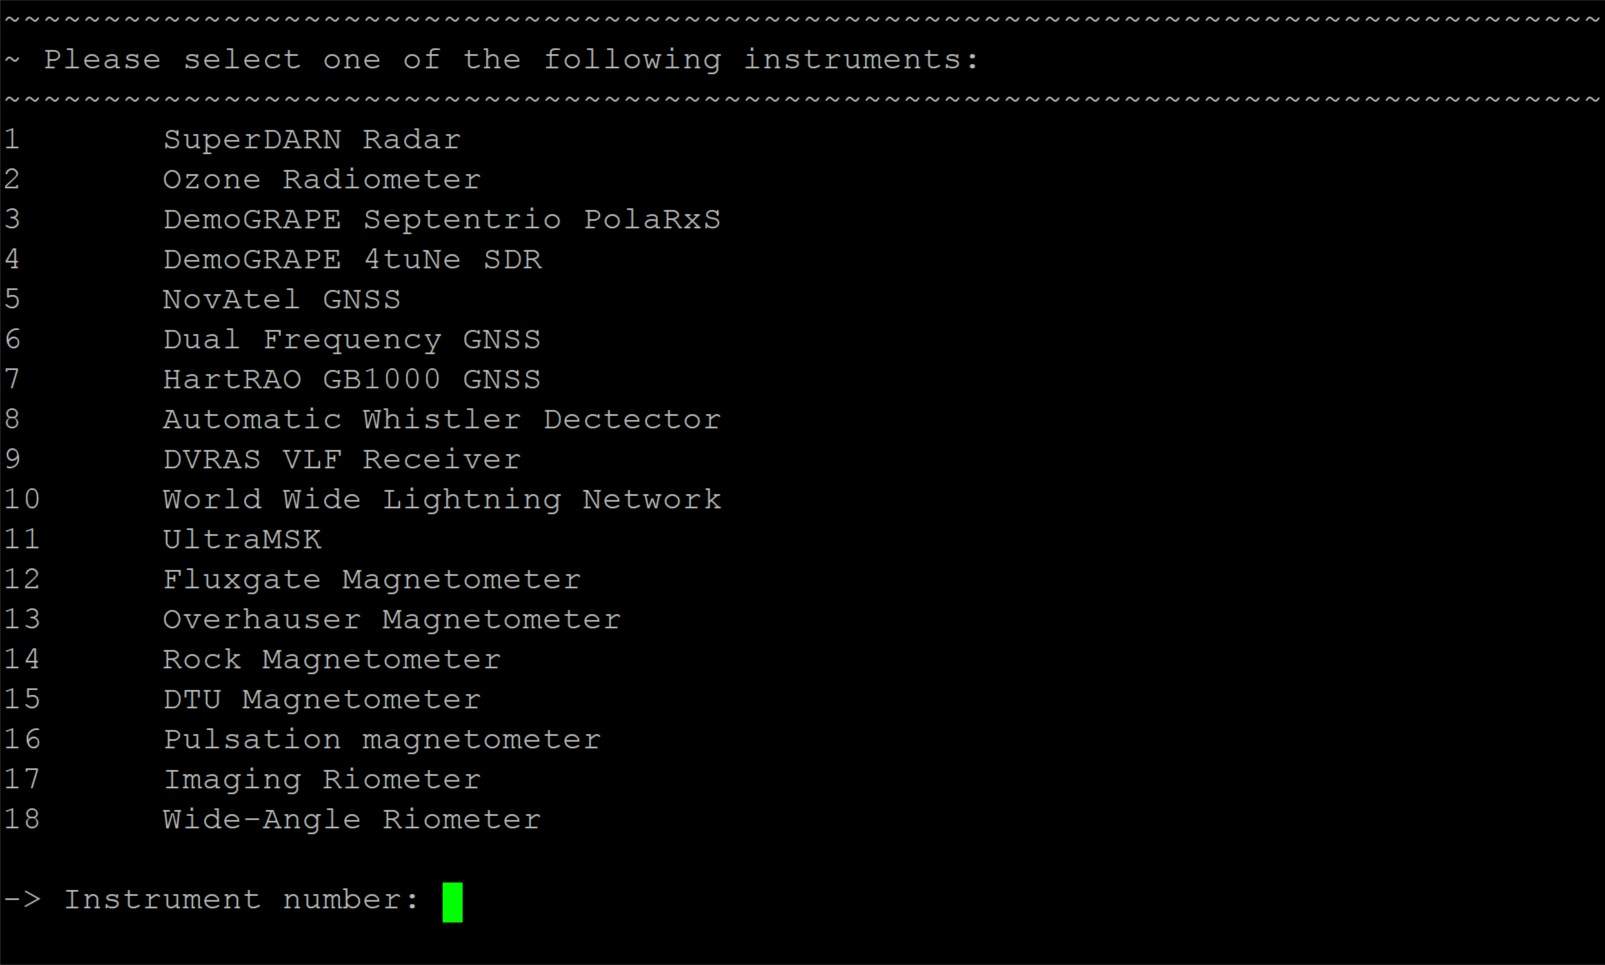
\includegraphics[width=0.7\textwidth]{images/operations/logger_1.jpg}
			\caption{Logging a new activity: Step 1.}
			\label{fig:ops_log1}
		\end{figure}
	\newpage
	\item The next prompt will ask for the name of the person responsible. A default name is displayed, which is read from the universal configuration file. To select the default option provided, simply press the \textbf{Enter} key. If the default name is incorrect, type in the desired name and press \textbf{Enter}.
		\begin{figure}[H]
			\centering
			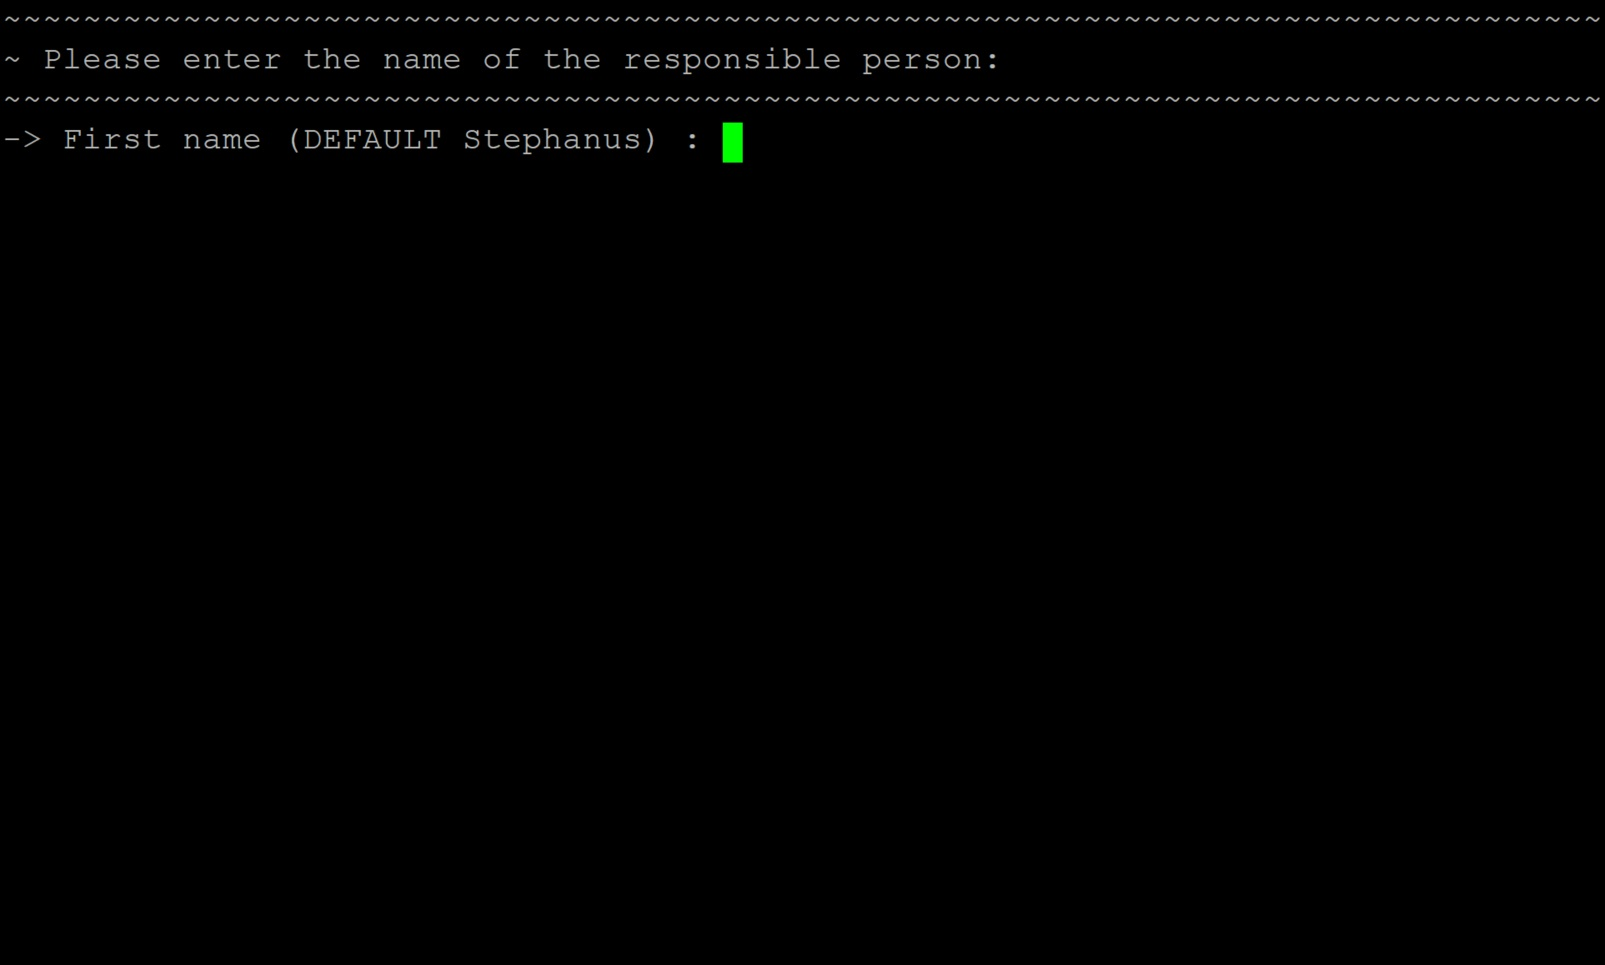
\includegraphics[width=0.7\textwidth]{images/operations/logger_2.jpg}
			\caption{Logging a new activity: Step 2.}
			\label{fig:ops_log2}
		\end{figure}
	\item When asked for the date, once again a default value is displayed. The default date is that of the present day and if the event occurred on a previous day, that date should be entered in the correct format.
		\begin{figure}[H]
			\centering
			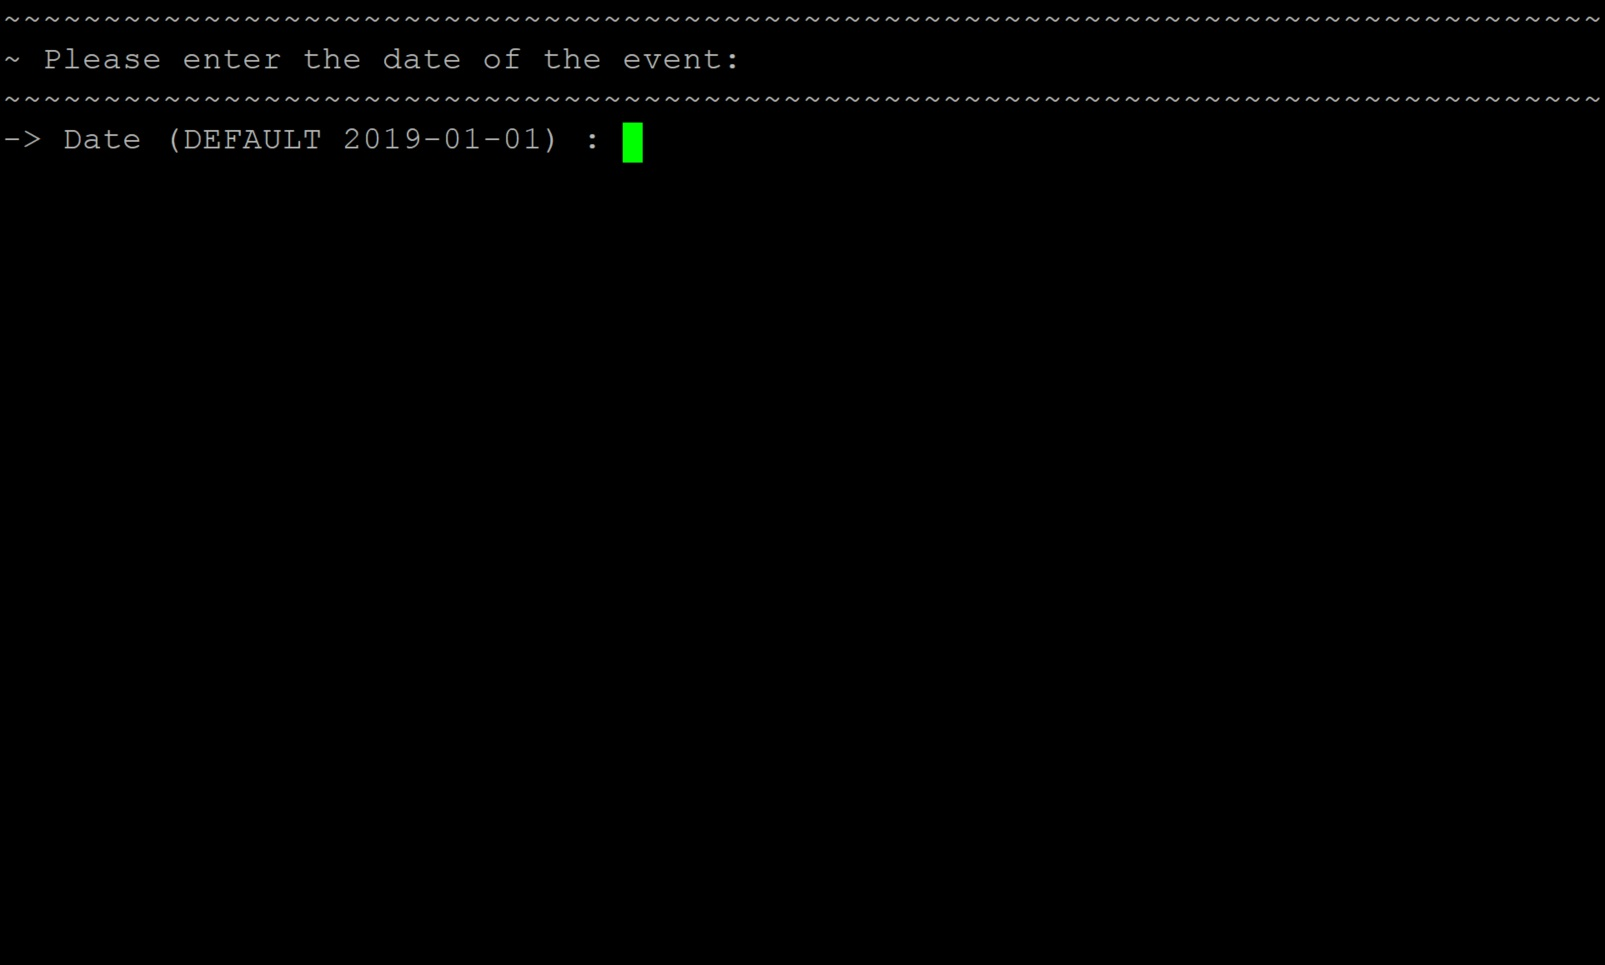
\includegraphics[width=0.7\textwidth]{images/operations/logger_3.jpg}
			\caption{Logging a new activity: Step 3.}
			\label{fig:ops_log3}
		\end{figure}
	\newpage
	\item The time is then prompted, once again with the current time as default. Press \textbf{Enter} or type in the desired time for the event.
		\begin{figure}[H]
			\centering
			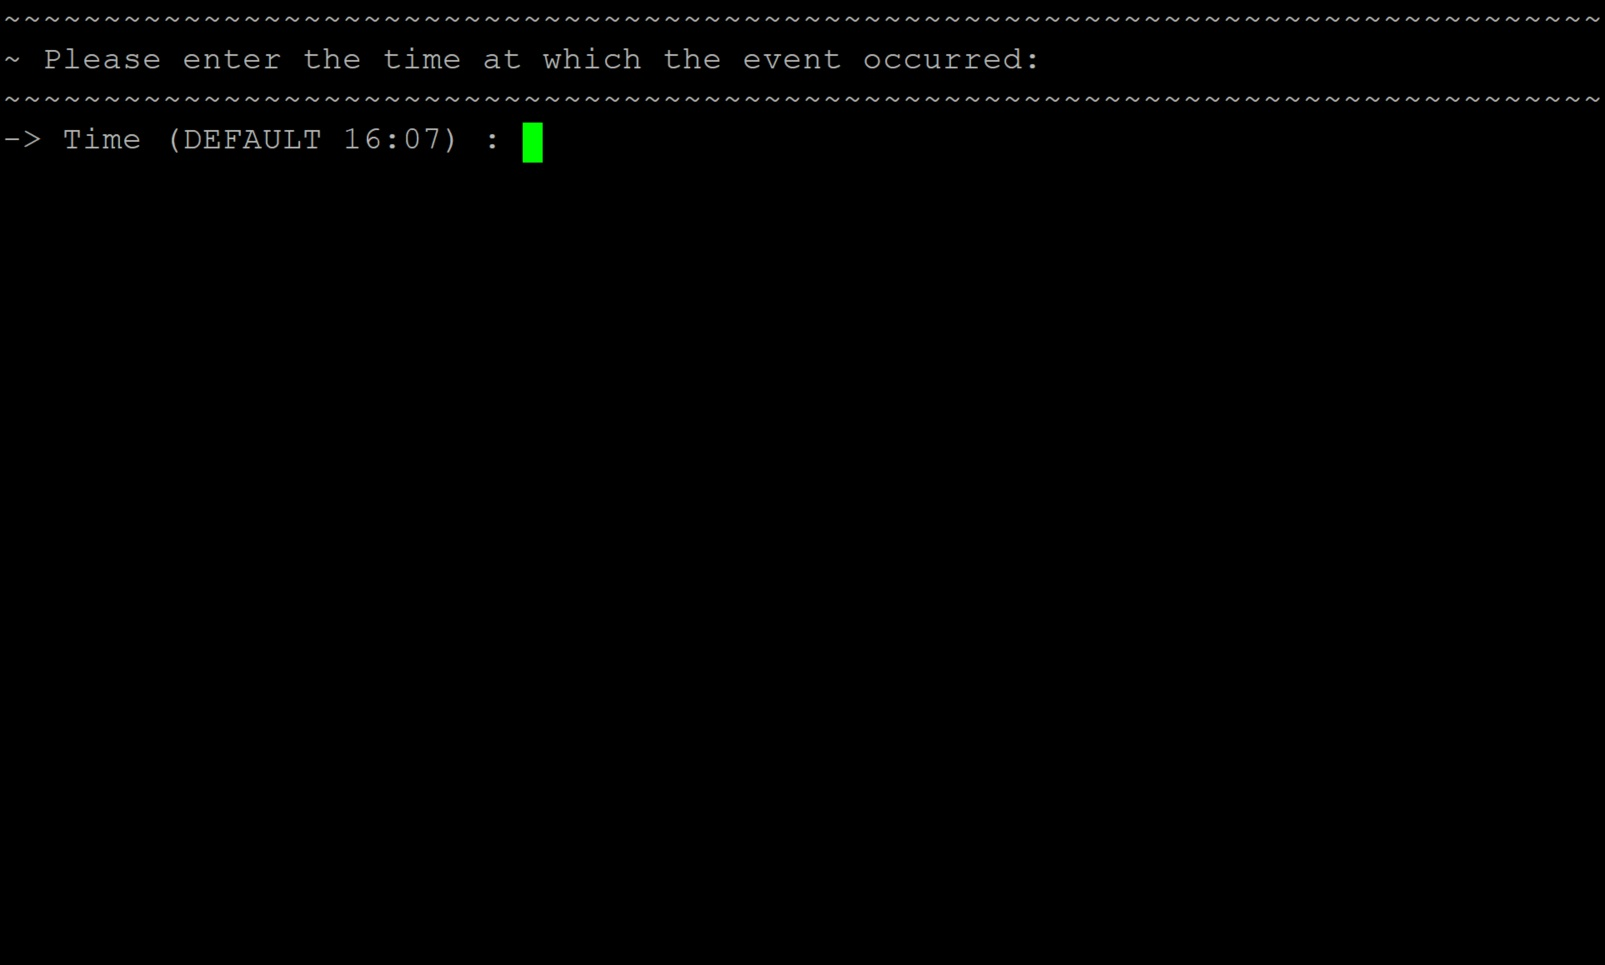
\includegraphics[width=0.7\textwidth]{images/operations/logger_4.jpg}
			\caption{Logging a new activity: Step 4.}
			\label{fig:ops_log4}
		\end{figure}
	\item The new status of the system can then be selected from a list of options. These include 0 (the system is off and no data is being logged), 1 (the system is logging data, but interference caused it to be invalid) and 2 (the system is up and logging valid data). Select one of these options and press \textbf{Enter}.
		\begin{figure}[H]
			\centering
			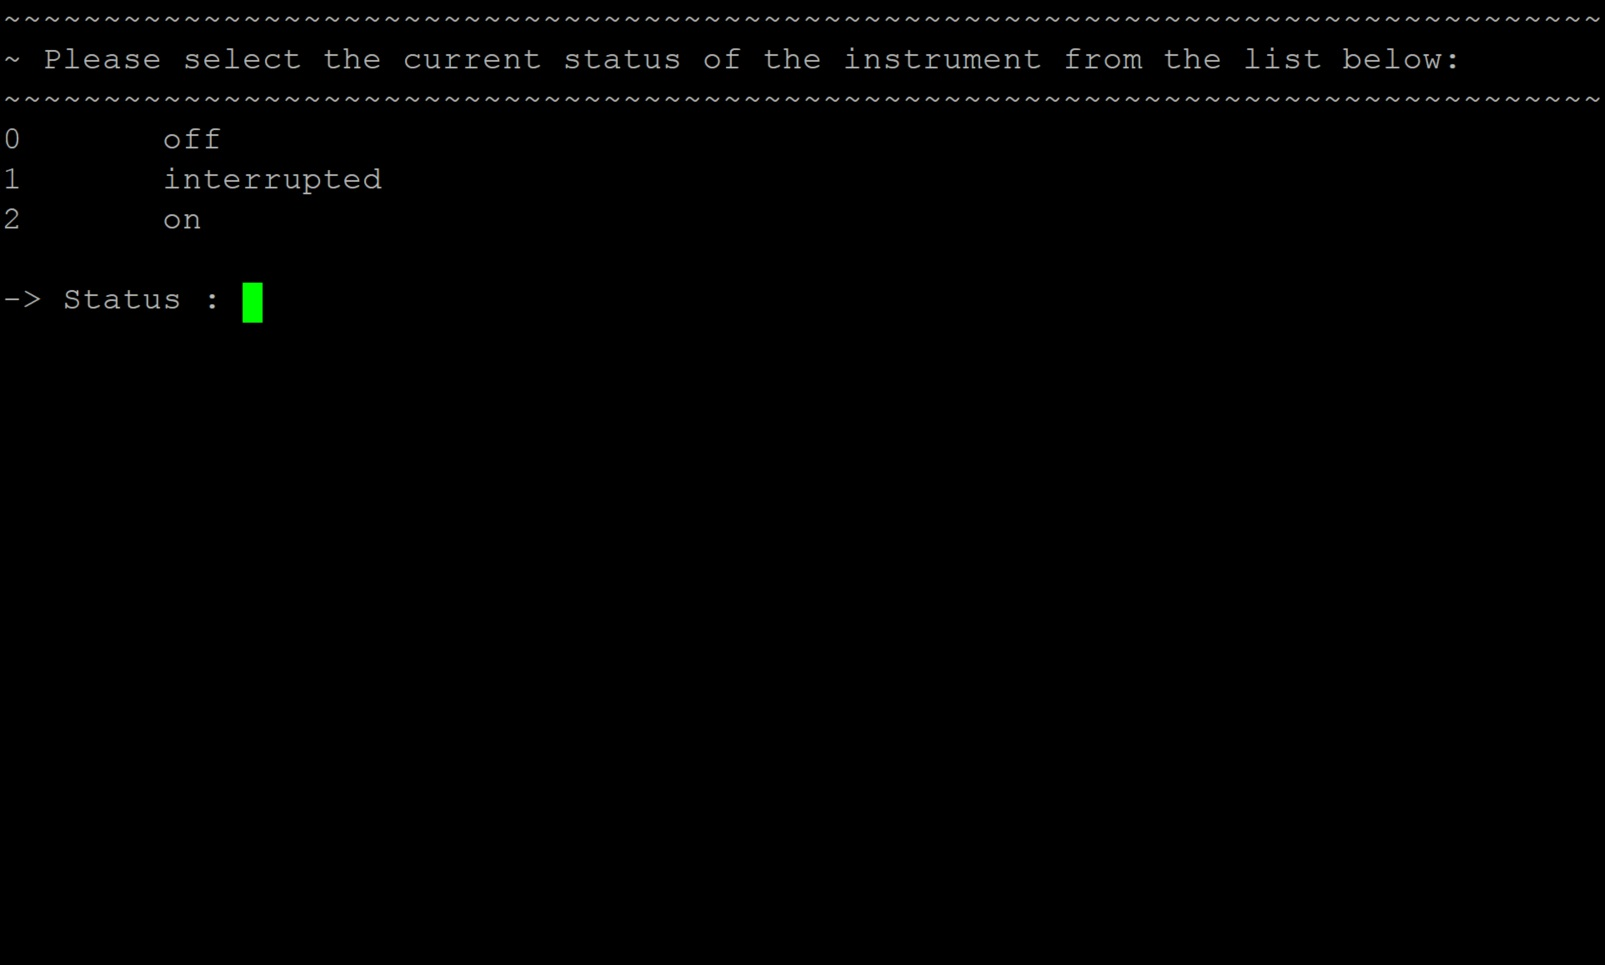
\includegraphics[width=0.7\textwidth]{images/operations/logger_5.jpg}
			\caption{Logging a new activity: Step 5.}
			\label{fig:ops_log5}
		\end{figure}
	\newpage
	\item Finally, the user is asked to elaborate on the reason behind the event. Provide as much information as possible, typing in full sentences. Avoid using special characters as part of this entry. When done, press \textbf{Enter} and wait for the logs to be synchronized and uploaded to the influxDB database.
		\begin{figure}[H]
			\centering
			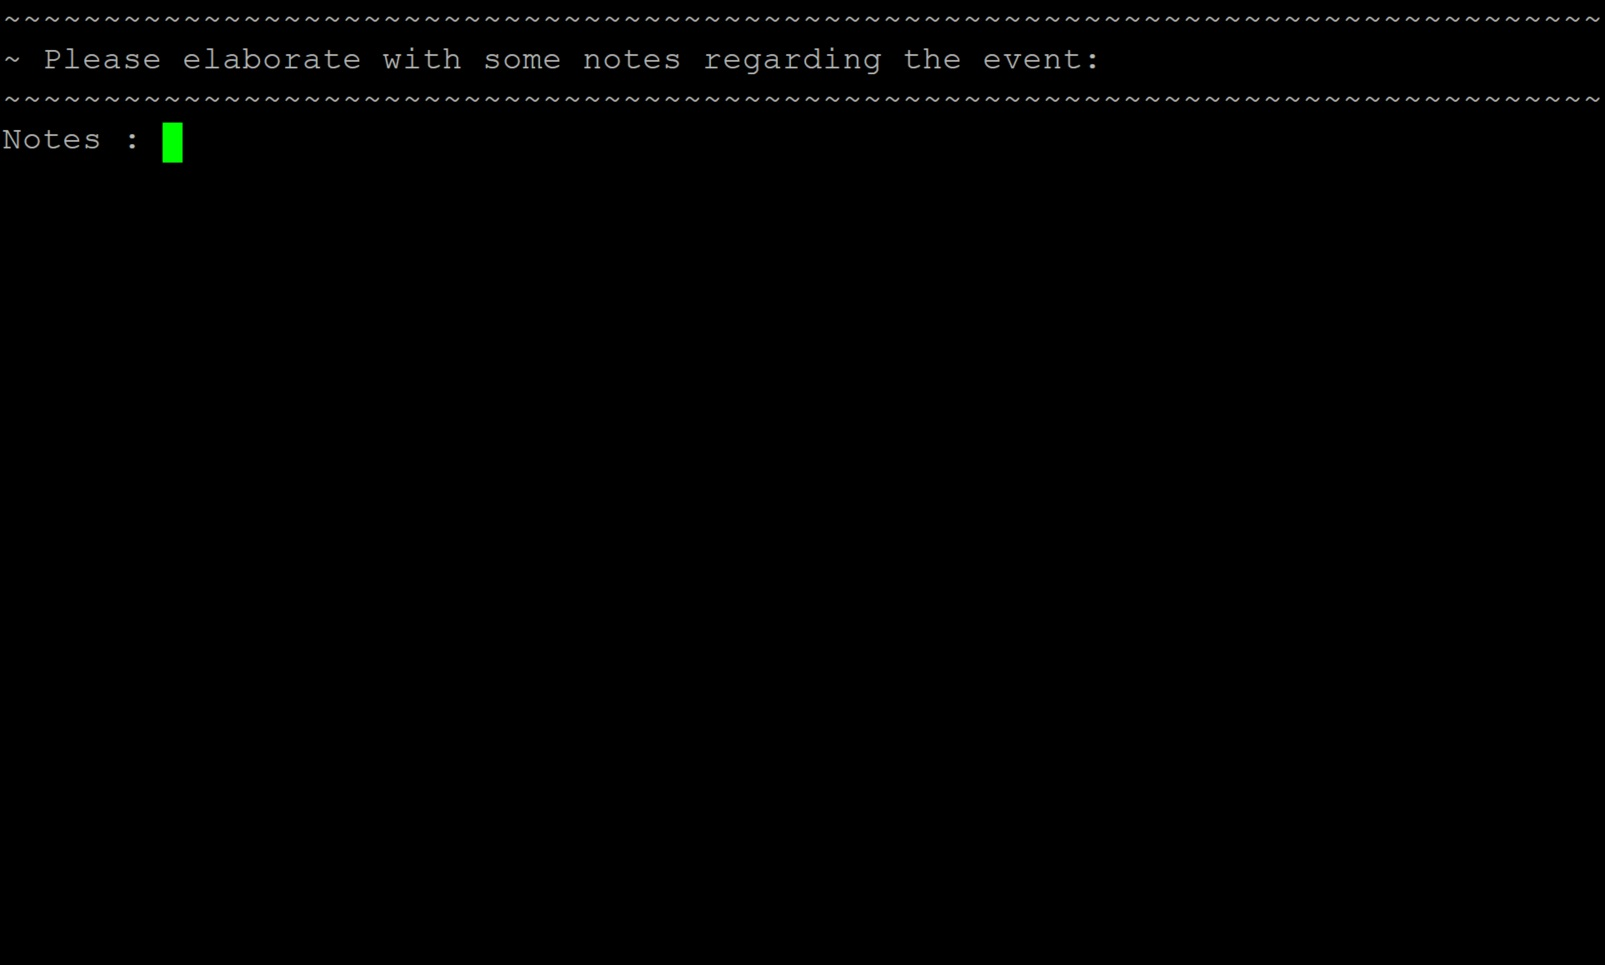
\includegraphics[width=0.7\textwidth]{images/operations/logger_6.jpg}
			\caption{Logging a new activity: Step 6.}
			\label{fig:ops_log6}
		\end{figure}
\end{enumerate}

\subsubsection{Deleting an Activity}
To delete a faulty activity entry, run the script: \textbf{del.sh} and follow the instructions, as demonstrated by the following steps:

\clearpage

\begin{enumerate}
	\item First, the script will display an enumerated list of all the registered systems. It will then prompt for an instrument number, corresponding to the instrument on which the activity is to be logged. Enter the number and then press the \textbf{Enter} key.
		\begin{figure}[H]
			\centering
			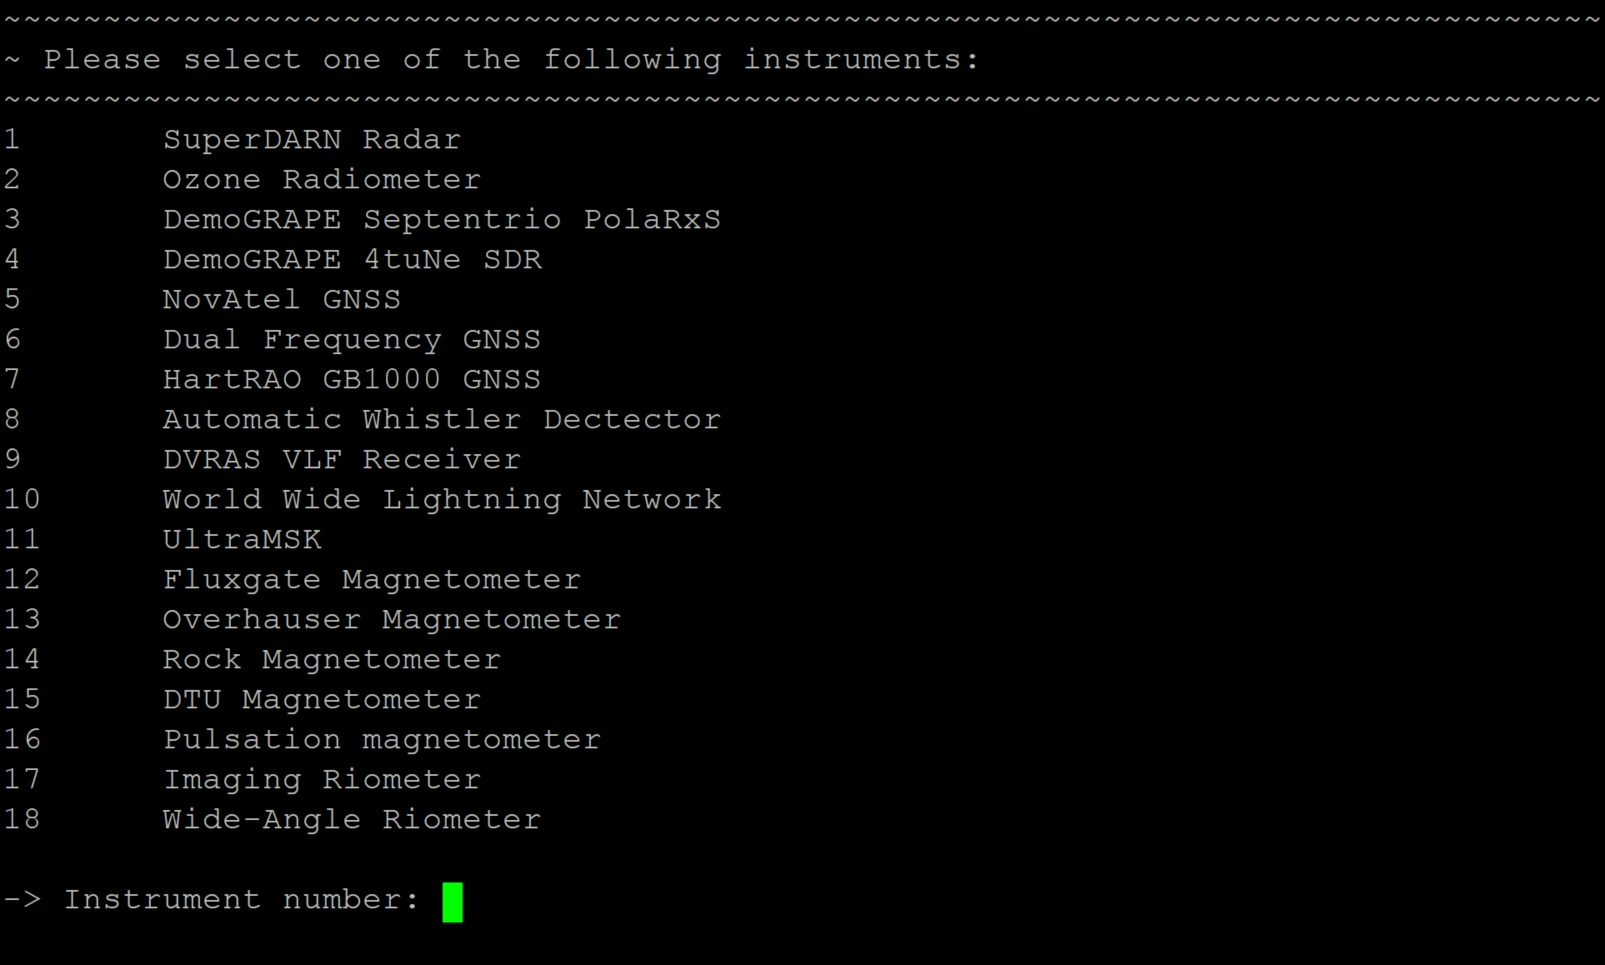
\includegraphics[width=0.7\textwidth]{images/operations/delete_1.jpg}
			\caption{Deleting an activity: Step 1.}
			\label{fig:ops_del1}
		\end{figure}
	\item When asked for the date, once again a default value is displayed. The default date is that of the present day and if the event occurred on a previous day, that date should be entered in the correct format.
		\begin{figure}[H]
			\centering
			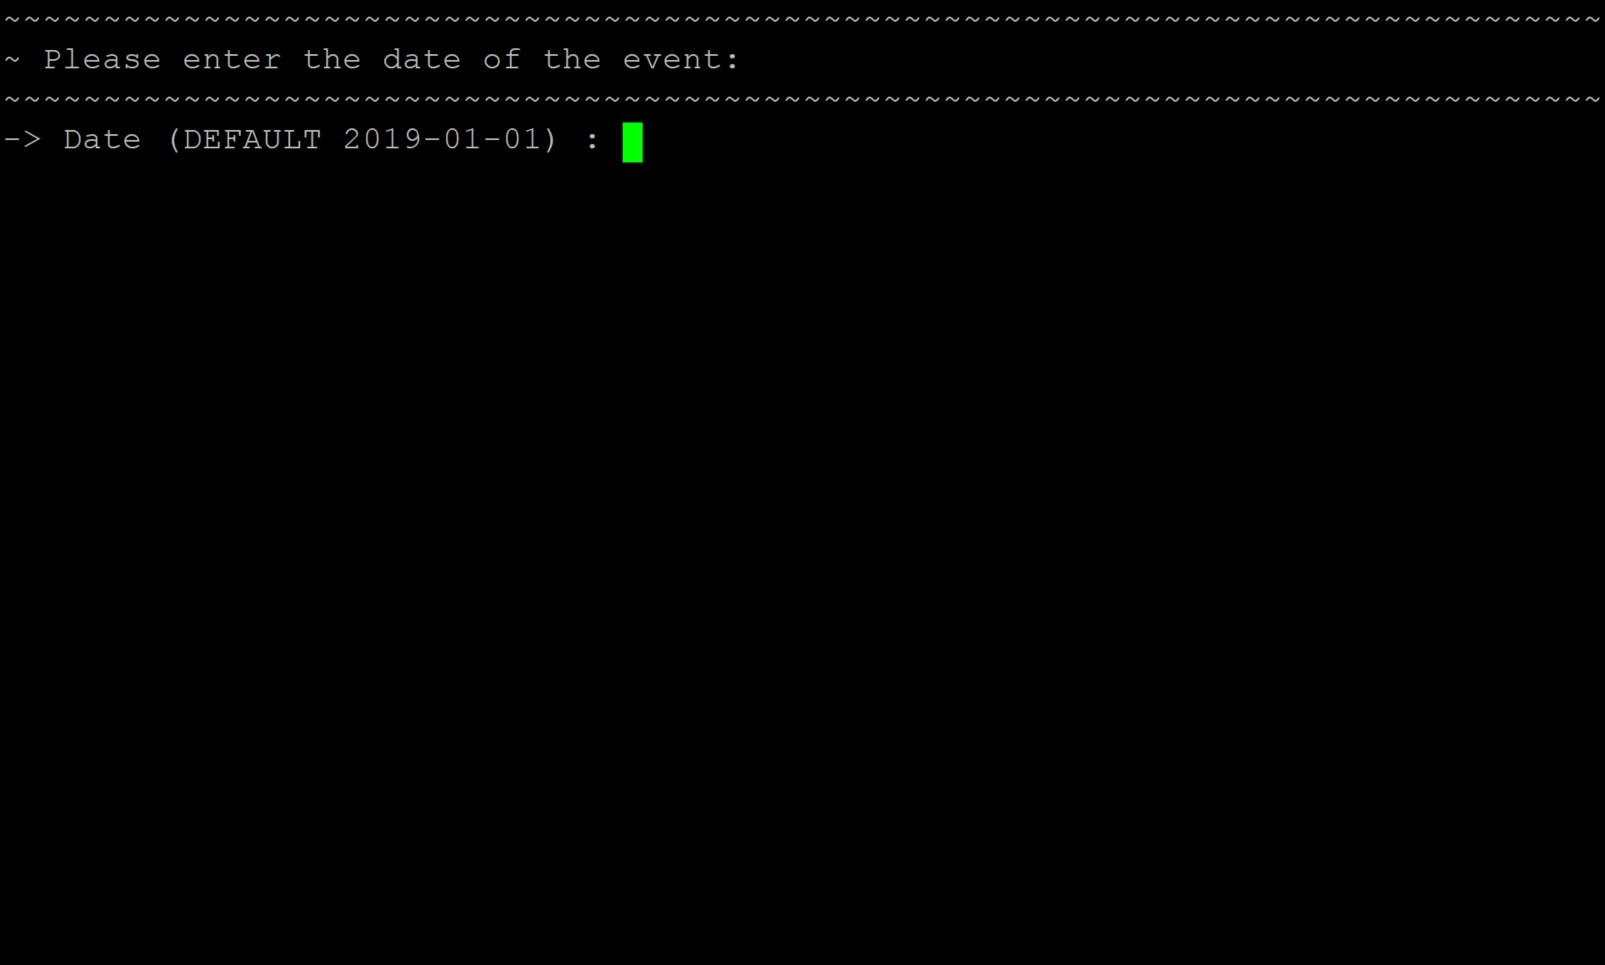
\includegraphics[width=0.7\textwidth]{images/operations/delete_2.jpg}
			\caption{Deleting an activity: Step 2.}
			\label{fig:ops_del2}
		\end{figure}
	\newpage
	\item The script will then display an enumerated list of all the activities logged for the date previously specified. Enter the number corresponding to the faulty entry and press \textbf{Entry} to delete that entry. Wait for the logs to be synchronized with the instrument PC and influxDB database.
		\begin{figure}[H]
			\centering
			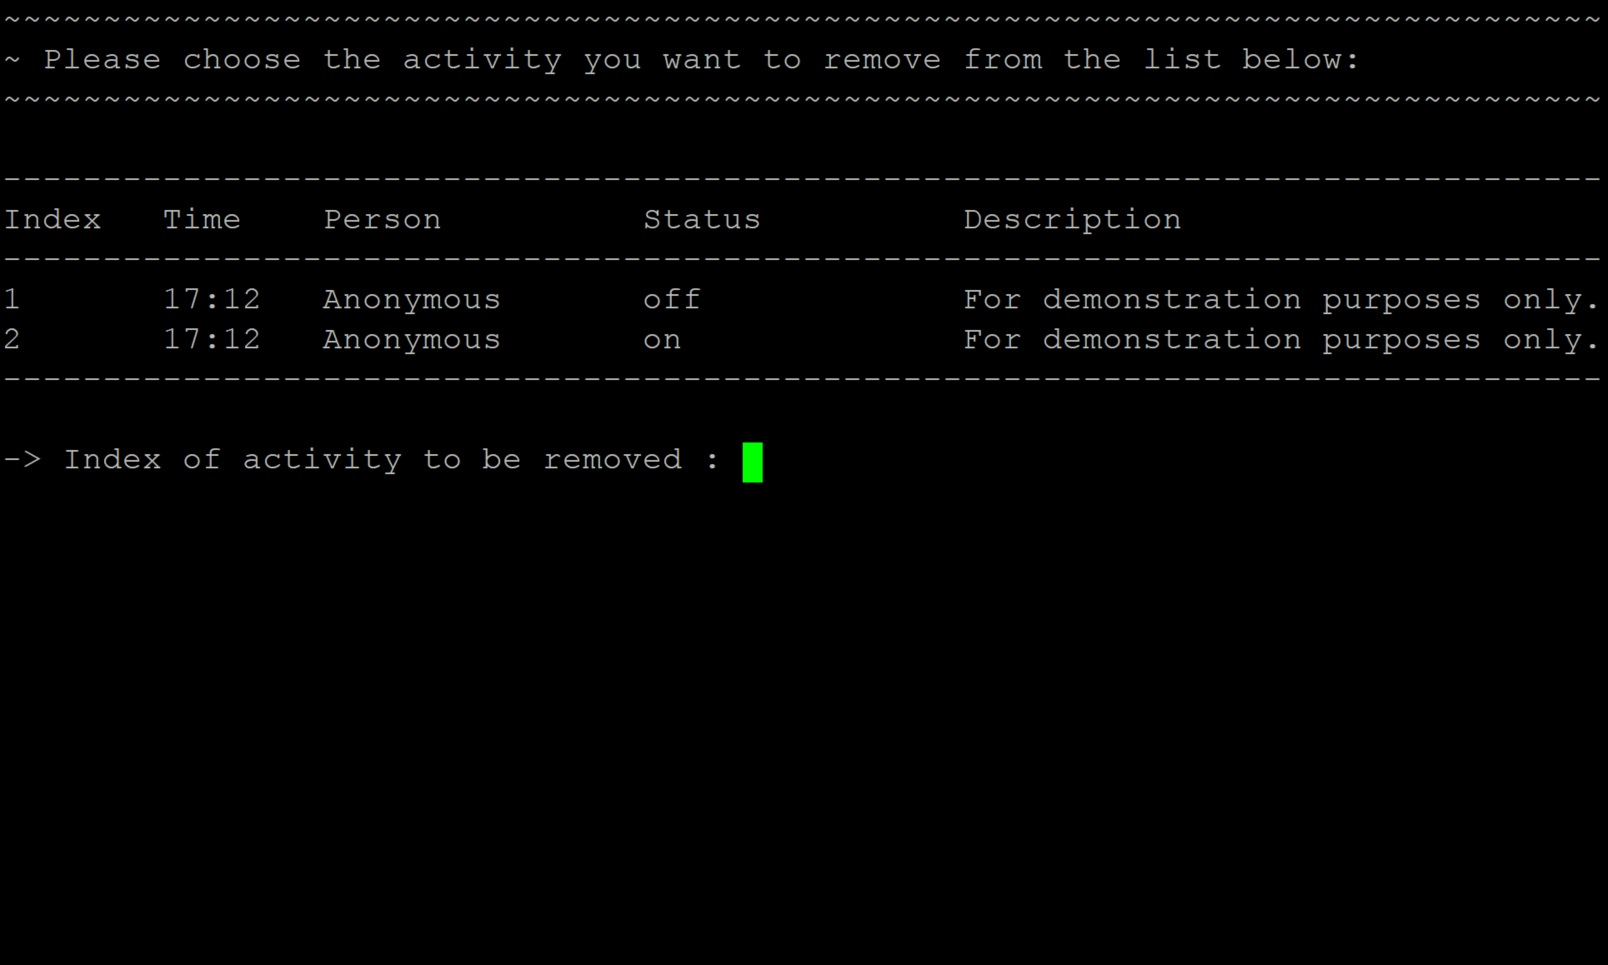
\includegraphics[width=0.7\textwidth]{images/operations/delete_3.jpg}
			\caption{Deleting an activity: Step 3.}
			\label{fig:ops_del3}
		\end{figure}
\end{enumerate}

\subsubsection{Adding a New Instrument}

\clearpage

\subsection{Monitoring}
\label{subsec:ops_monitoring}
A live monitoring system for all of the instruments on base have been implemented in Grafana, working with an InfluxDB back-end. This section explains how this system works, from the data collection scripts, reading data into the InfluxDB databases and displaying the data and statistics on a Grafana dashboard.

\subsubsection{Overview}
For each system, data is transferred to the data server at set intervals. These intervals can be seen and set in the crontab of the data server. The data collector script, which is called by the crontab, runs a datacrawler script on the instrument PC via ssh. These datacrawlers are responsible for reading the most recent data and formatting it to comply with the influxDB Line Protocol. The file containing the database entries is then transferred to data server, from where it is read into the influxDB database. Refer to \figref{ops_monitoring} below.
\par
\begin{figure}[H]
	\centering
	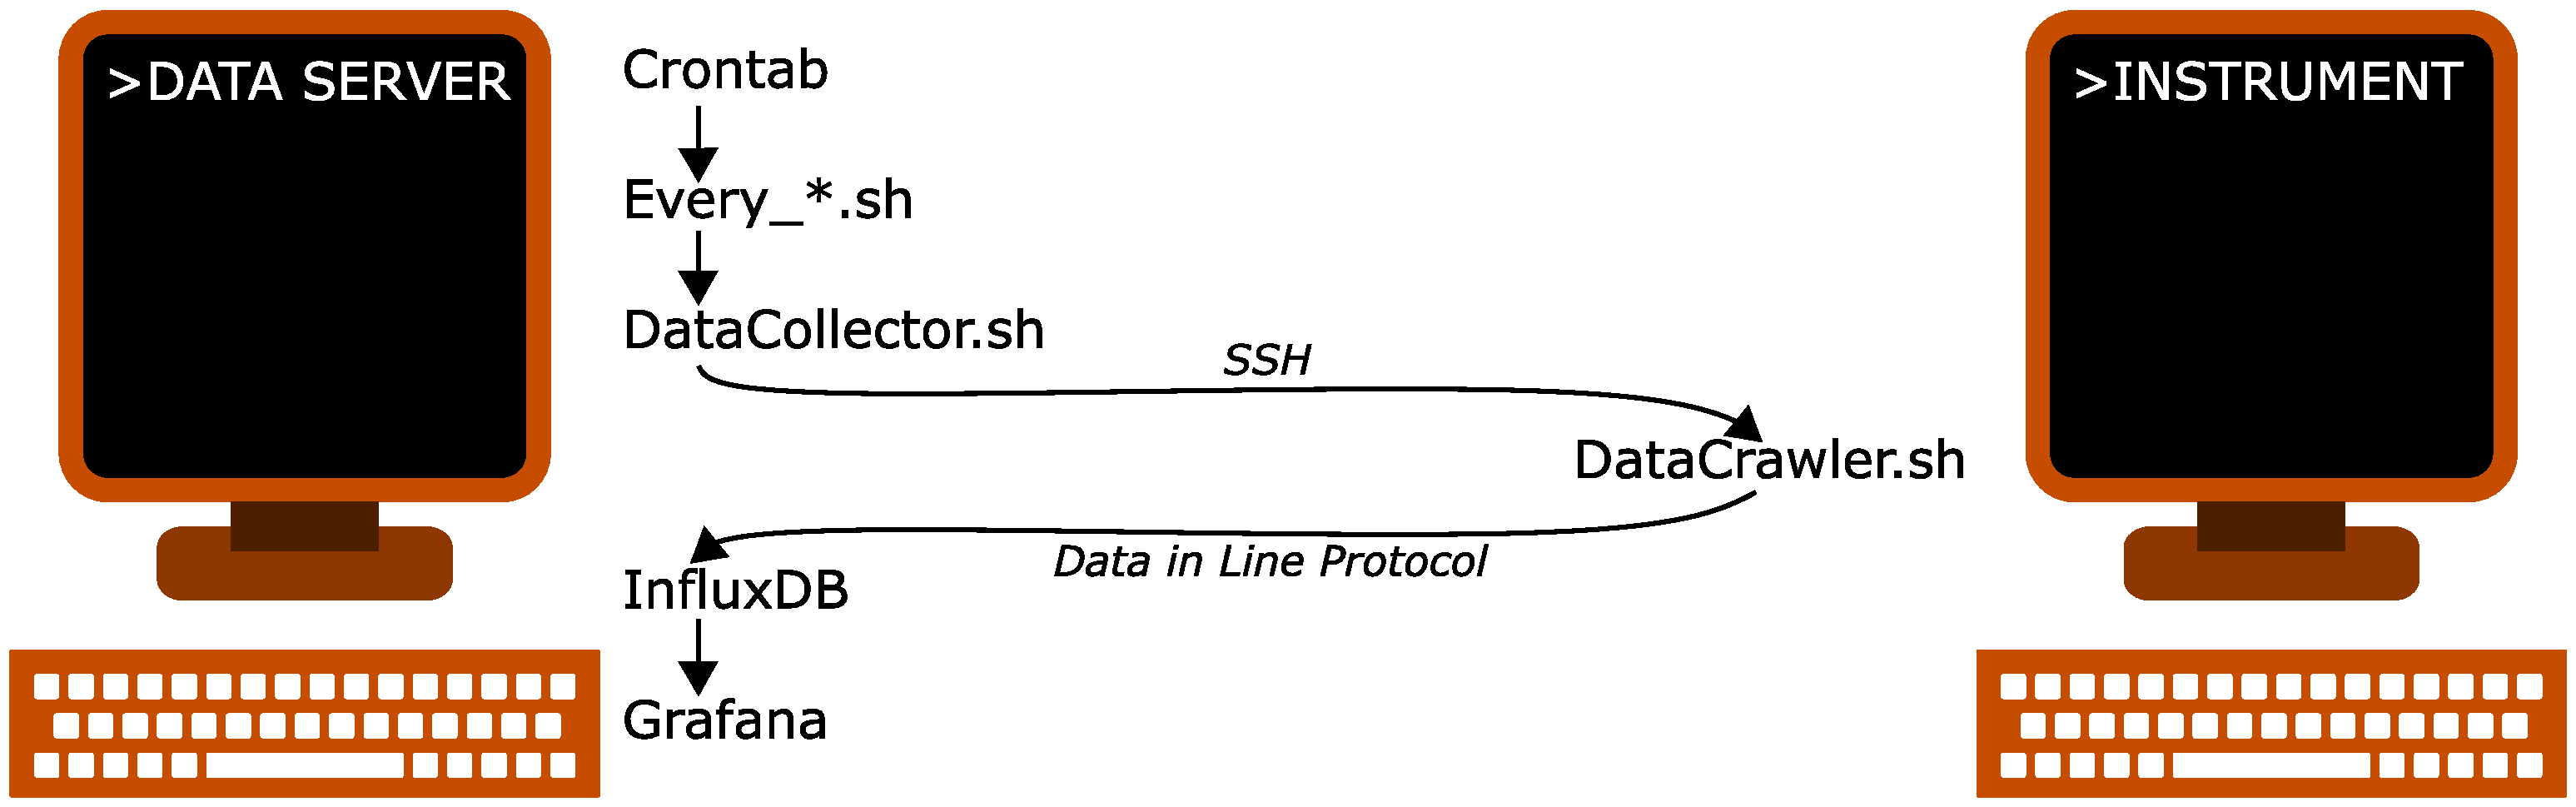
\includegraphics[width=\textwidth]{images/operations/grafana_graphic.pdf}
	\caption{Monitoring System Overview.}
	\label{fig:ops_monitoring}
\end{figure}

Graph and explanation of datacollector, datacrawler, influx, grafana, etc.

\subsubsection{Scripts}
\subsubsection{Backfilling}
\subsubsection{InfluxDB}
\subsubsection{Grafana}

scripts, data, backfilling, influx commands, retention policy

\clearpage

\subsection{Reporting}
\label{subsec:ops_reporting}
script and how to copy to desktop. (Luatex for memory problems)


\clearpage